\section{Tables}

Example of a complex, nicely formatted table is given in \autoref{tab:pretty}.

\begin{table}[t]
  \centering
  \footnotesize
  % Tweak the tabcolsep if desired if a table looks awkward.
  % \setlength{\tabcolsep}{3pt}
  \caption{My table's caption.}
  \label{tab:pretty}
  % Tabularx lets us explicitly set the table width
  % If using tabularx, X is a good column specifier for text.
  % S is a great column specifier for numeric data. It's provided by the siunitx
  % package.
  % The @{} token can be used anywhere in the column list to remove padding, if
  % desired.
  \begin{tabularx}{\columnwidth}{XSSS}
    \toprule
    \multirow{2}{*}{Label} & \multicolumn{2}{c}{X} & Y \\
    \cmidrule(lr){2-3} \cmidrule(lr){4-4}
                           & A & B & C \\
    \midrule
    Foo & 3.14 & 1 & 1e4 \\
    Bar & 31.4 & 1000 & 1e-4\\
    Baz & .314 & 100000 & 5\\
    \bottomrule
  \end{tabularx}
\end{table}

\section{Numbers}

\begin{itemize}
  \item A pretty fraction: \sfrac{1}{2}
  \item A pretty number: \num{123456}. Using the num macro is better than doing
    it yourself, as some fonts insert a small space after the comma: 123,456.
  \item Some typefaces distinguish numbers used in text from numbers used in
    math mode. Try to be careful to treat numbers in the English language
    (e.g., 5~dogs) differently than math $5 \times 5$.
\end{itemize}

\section{Math}
\begin{itemize}
  \item \textbf{Never} use a string of characters in math mode: $aes256(\cdot)$.
    Instead, consider using \texttt{DeclareMathOperator} in the preamble:
    $\aes(\cdot)$. Common operators are available: $\log$, $\sin$, $\Pr$, etc.
  \item If you have a variable that has multiple characters but is not an
    operator, typeset with \texttt{mathit}: $\mathit{TPR}$ (spacing is correct
    v.s. $TPR$).
  \item $\varepsilon$ is probably the epsilon character you're looking for, not
    $\epsilon$. You might also want $\varphi$ instead of $\phi$.
  \item \texttt{mathbbm} offers alternatives you may prefer to the common
    \texttt{mathbb} set typography 
    $\mathbb{N, R, Z}$: $\mathbbm{N, R, Z}$.
  \item Use paired delimiters for correct sizing: $\left( x \right)$.
\end{itemize}

\section{References and Citations}
\label{sec:refs}

\subsection{In-Paper References}
\label{subsec:in-paper}

Autoref does the hard work of referencing things for you:
\autoref{tab:pretty}, \autoref{fig:cat}, \autoref{eq:gauss}, \autoref{sec:refs},
\autoref{subsec:in-paper}. Reference styles can be controlled 

\begin{figure}[t]
  \centering
  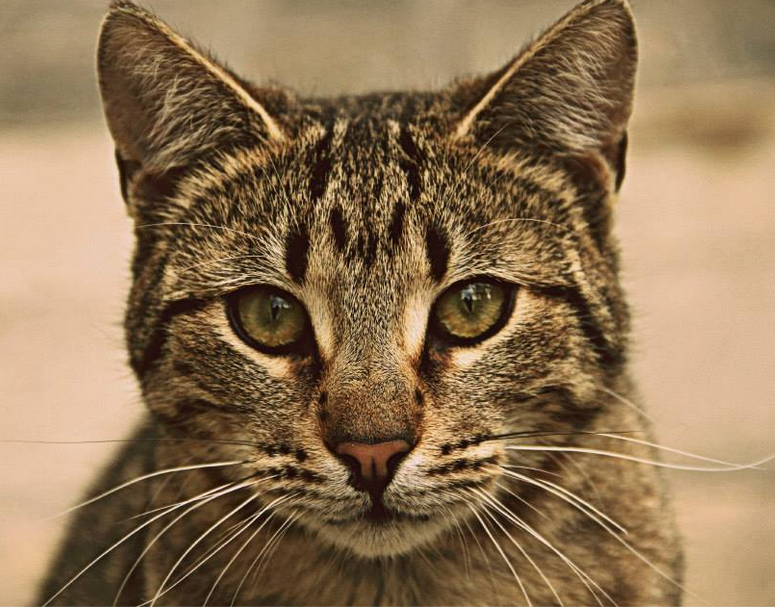
\includegraphics[width=\columnwidth]{cat.png}
  \caption{Felis catus}
  \label{fig:cat}
\end{figure}

\begin{equation}
  \nabla \cdot \bm{E} = \frac{\rho}{\varepsilon_0}
  \label{eq:gauss}
\end{equation}

\subsection{External References}

Use \texttt{citeauthor} to get the list of authors for a reference:
\citeauthor{TIT:DiffieH76}~\cite{TIT:DiffieH76}.
For a list of more than two authors, \texttt{citeauthor*} can be used to get the
standard et al. string:
\citeauthor*{JMLR:PedregosaVGMTGBPWDVPCBPD11}.

Biblatex handles online (\texttt{@online}) references nicely:
\cite{bhattacharyya}. Bib entries with a \texttt{DOI} entry have a handy link
that goes right to the document.
